\chapter{Co-optimised Energy Arbitrage with Regulation Participation}
\label{sec:coop_method}
As discussed in Section \ref{cooptimisation}, co-optimisation between regulation markets and energy arbitrage revenue has little supporting literature, only explored in the NEM by \parencite{Zhai:2018}. \parencite{McConnell} discarded the idea of co-optimisation in 2015, deeming the FCAS market \textit{``very small relative to the wholesale market''} and arguing \textit{``ancillary market as it is not expected to have a measurable impact
on the results''}. However, in 2016, for system security purposes, AEMO required the local procurement of 35 MW of Regulation FCAS in South Australia at times when the separation of the region at the Heywood interconnector was a credible contingency. During these times of local requirements, FCAS prices were very high due to the
limited number of suppliers of these services, as shown in Figure \ref{fig:fcas_prices}. AEMO estimates that the 35 MW FCAS constraint added more than \$100 million in FCAS costs over 2016 and 2017, withdrawing it on the October 12, 2018. 
\begin{figure}[H]
    \centering
    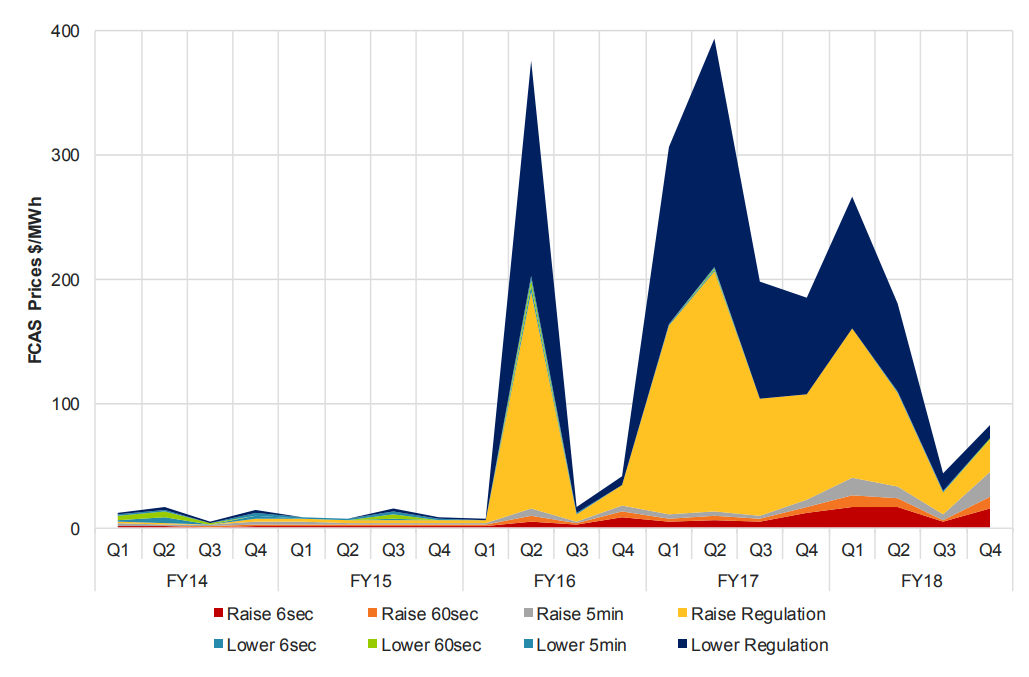
\includegraphics[width=0.6\textwidth]{Pictures/Chapter6/reg_prices.PNG}
    \caption{Quarterly average South Australian FCAS prices by service \parencite{sa_aemo}}
    \label{fig:fcas_prices}
\end{figure}
The implication of such high prices in the ancillary service market has driven a heightened interest in optimising BESS dispatch across energy and FCAS services. \section{ Methodology }
This thesis explores co-optimisation of energy and regulation FCAS participation via a novel technique developed by Daniel Tam (co-author). Recapping \ref{cooptimisation}, the regulation FCAS market consists of both raise and lower services, offered as a deviation from the set-point dictated by the energy market. Under current market arrangements, generators may be enabled for both raise and lower regulation services at the same time as offering bulk energy services. As such, a complete optimisation can be formed as the linear program below:
\begin{align*}
  \max \sum_{i=0}^T 
   \left[  \left(x^{(i)}_c + x^{(i)}_d - (x^{(i)}_{l_g} + x^{(i)}_{l_l}) k^{(i)}_l + (x^{(i)}_{r_g} + x^{(i)}_{r_l}) k^{(i)}_r\right) p_{e}^{(i)} \
    + (x^{(i)}_{l_g} + x^{(i)}_{l_l}) p_{l}^{(i)} +(x^{(i)}_{r_g} + x^{(i)}_{r_l}) p_r^{(i)}  \right] \times \left( \frac{l}{60} \right)
\end{align*}
Subject to the constraints:
\begin{alignat*} {3}
    -P_{max} &\leq x^{(i)}_c \leq 0  &&\forall i \in [0,T] \hspace{1cm} &&  \text{(Charge Power Capacity)}\\
    0 &\leq x^{(i)}_d \leq P_{max}  &&\forall i \in [0,T] && \text{(Discharge Power Capacity)}\\
    0 &\leq x^{(i)}_{l_g} \leq x^{(i)}_d  &&\forall i \in [0,T] && \text{(Generator Lower Availability)}\\
    0 &\leq x^{(i)}_{r_g} + x^{(i)}_d\leq  P_{max} \hspace{1cm} &&\forall i \in [0,T] && \text{(Generator Raise Availability)}\\
    0 &\leq x^{(i)}_{l_l} -  x^{(i)}_c\leq P_{max}  &&\forall i \in [0,T] && \text{(Load Lower Availability)}\\
    0 &\leq x^{(i)}_{r_l}  \leq -x^{(i)}_c  &&\forall i \in [0,T] && \text{(Load Raise Availability)}\\
    0 &\leq E^{(i)} \leq E_{max} &&\forall i \in [0,T] && \text{(Storage Capacity)} \\
\end{alignat*}
Initial Storage Capacity:
\begin{align*}
    E^{(0)} &= E_{\text{init}} - 
     \left( 
        \left(x^{(0)}_c - x^{(0)}_{l_l} k^{(0)}_l + x^{(0)}_{r_l} k^{(0)}_r   \right) \eta_c + 
        \left(x^{(0)}_d - x^{(0)}_{l_g} k^{(0)}_l + x^{(0)}_{r_g} k^{(0)}_r\right) \frac{1}{\eta_d} 
    \right)
   \frac{l}{60}
\end{align*}
Temporal Storage Link:
\begin{align*}
E^{(i)} &= E^{(i-1)} - 
     \left( 
        \left(x^{(i)}_c - x^{(i)}_{l_l} k^{(i)}_l + x^{(i)}_{r_l} k^{(i)}_r   \right) \eta_c + 
        \left(x^{(i)}_d - x^{(i)}_{l_g} k^{(i)}_l + x^{(i)}_{r_g} k^{(i)}_r\right) \frac{1}{\eta_d} 
    \right)
   \frac{l}{60} \hspace{0.5cm} \forall i \in [0,T]
\end{align*}
Where,
{\renewcommand{\arraystretch}{2}}
\begin{center}
    \begin{table}[H]
        \small
        \centering
        \begin{tabular}{p{0.8cm} p{6.4cm} p{0.8cm} p{6.4cm}}
        \textbf{Constants} & & \textbf{Variables} & \\
        $P_{max}$ & Power Capacity of BESS (MW) & $x^{(i)}_c$ & Charge power at time $i$ (MW)   \\ 
        $E_{max}$ & Storage Capacity of BESS (MWh) & $x^{(i)}_d$&  Discharge power at time $i$ (MW)  \\
        $E_{\text{init}}$ & Initial Storage Level of BESS (MWh)& $E^{(i)}$ &Storage level at time $i$ (MWh)\\
        $l$ & length of time interval in minutes & $x_l^{(i)}$ & Enabled lower regulation at time $i$ (MW)\\
        $\eta_c$ & Charge efficiency (\%) & $x_r^{(i)}$ & Enabled raise regulation at time $i$ (MW)\\
        $\eta_d$ & Discharge efficiency (\%) & &\\
        $p_e^{(i)}$ &  Energy price at time $i$ (\$/MWh) & &\\
        $p_l^{(i)}$ &  Lower regulation price at time $i$ (\$/MW/h) & &\\
        $p_r^{(i)}$ &  Raise regulation price at time $i$ (\$/MW/h) & &\\
        $k^{(i)}_l $ & Lower throughput at time $i$ (\%) & & \\
        $k^{(i)}_r$ & Raise throughput at time $i$ (\%) & & \\
        $T$ &  Total number of time intervals & &\\
        \end{tabular}
        \label{tab:my_label}
    \end{table}
\end{center}
\subsection{  Impact of Energy Throughput During Regulation Participation }
As discussion in Section \ref{cooptimisation}, the FCAS market participants are paid for the reserves offered to AEMO if they are not instructed to alter the power dispatch level. Once the instructions are issued, they are also paid or need to pay for the amount of energy delivered or received at the spot trading price. The FCAS instruction is termed “AGC energy delivered”. The following quote is an except from \parencite{Zhai:2018}.

\begin{tcolorbox}[colback=ocre!5!white,colframe=ocre]
\textit{``It is worth noting that even if the battery did not make offers in the spot market and participated in the FRS markets only, \textbf{there is still a spot market revenue stream due to the AGC energy dispatched for the FRS offers}. It means that the spot trading prices still need to be watched carefully for the battery operating in the FRS markets only, in order to maximize its profit.}" (Zhai, 2018)
\end{tcolorbox}
Due to this phenomenon, the algorithm above includes the terms $k_1$ and $k_r$, which refers to the percentage of energy which is throughout relative to the enabled regulation $x_l$ and $x_r$ for a given period. To determine these percentages, one must look at the 4 second interval data published by AEMO via NEMWEB under the causer pays data. During the initial trial of the Hornsdale Power Reserve for the period 10th December 2017 to 7th January 2018, AEMO provided the Regulation MW component of the zip in a separate location available here: \url{https://www.aemo.com.au/Electricity/National-Electricity-Market-NEM/Data/Ancillary-Services/Ancillary-Services-Market-Causer-Pays-Data}
Due to the shear amount of data in the causer pays data, AEMO only keeps the last 60 day on NEMWEB before purging it. This data has been extracted and analysed as shown in Figure \ref{fig:agc_energy}. 
\begin{figure}[H]
    \centering
    \makebox[\textwidth][c]{    \includegraphics[width=\textwidth]{"Pictures/Chapter6/agc_througput".pdf}}
    \caption{AGC Energy Proportional Dispatch vs. Regulation Enablement for Hornsdale Power Reserve (10/12/2017 - 7/01/2018) }
    \label{fig:agc_energy}
\end{figure}
Figure \ref{fig:agc_energy} highlights that regulation raise is instructed via the AGC signal must more frequently than lower. As the AGC is inherently random as it is a stochastic output of the operating frequency of the grid, a Monte Carlo sampling approach has been used to determine the AGC energy component in the co-optimised model.  
\subsection{Analysis}
\subsubsection{Perfect Enablement}
In the NEM, 130 MW is procured for raise FCAS services while 120 MW is procured for FCAS lower services within a 5-minute dispatch interval. An accumulated time error of greater than ± 1.5 s may require additional regulation support of an extra 60 MW/s deviation for mainland. However, the linear program presented  in  Section  \ref{sec:coop_method},  assumes  the  BESS  as  an  FCAS  price-taker,  or  that  it  can  be  enabled  up  to its regulation availability at any point in time for the given price (perfect enablement). When dealing with energy arbitrage with small market price-taker assumption is generally accepted given the maximum demand typically sits around 3000MW, and minimum demand is close to 600MW \parencite{sa_aemo}. However given the size of the regulation markets, there are significant issues that arise if you maintain the price taker assumption. 

The results of the linear program for a 30MW/119MWh BESS in SA in 2018 are presented in Figure 5.3.  In this case we see regulation raise as the dominant revenue stream.  Interestingly,  the BESS energy setpoint alone (ie.what the battery is dispatched to provide in the energy market) would have provided negative revenue if dispatched in an energy only scenario.  Instead, the algorithm exploits the fact that revenue from the energy market is settledbased on metered actual values as opposed to energy setpoints.  Hence it positions itself to collect energy paytmentsfrom the net BESS output level determined by the superposition of the energy setpoint and the regulation AGCsignal.

\begin{figure}[H]
    \centering
    \makebox[\textwidth][c]{    \includegraphics[width=\textwidth]{"Pictures/Chapter6/monthly_perfectenablement".pdf}}
    \caption{Caption}
    \label{fig:my_label}
\end{figure}

\begin{figure}[H]
    \centering
    \makebox[\textwidth][c]{    \includegraphics[width=\textwidth]{"Pictures/Chapter6/monthly_10MW_perfectenablement".pdf}}
    \caption{Caption}
    \label{fig:my_label}
\end{figure}

\subsection{ Validation of Existing Asset Performance  }
\begin{figure}[H]
    \centering
    \makebox[\textwidth][c]{    \includegraphics[width=\textwidth]{"Pictures/Chapter5/Hornsdale Actual Monthly Energy & FCAS Revenue - South Australia 2018".pdf}}
    \caption{Caption}
    \label{fig:my_label}
\end{figure}